\subsection{Proposal result}
\subsubsection{Correlation of {\model} and semantic scores}
To evaluate the effectiveness {\model} compared to BLEU, we conducted experiments 
in the same manner with BLEU on three models lpSMT and mppSMT. 
%{\model}'s efficiency was tested on a large number
%of methods translated by those models. 

\begin{figure}[t]
\caption{{\model} vs semantic score (lpSMT)}
\centering
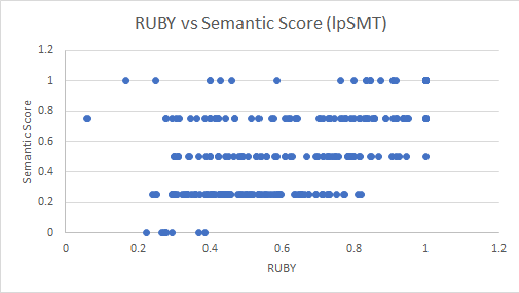
\includegraphics{img/rubyvssem_lpSMT.png}
\label{fig:RubySemlpSMT}
\end{figure}

\begin{figure}[t]
\caption{{\model} vs semantic score (mppSMT)}
\centering
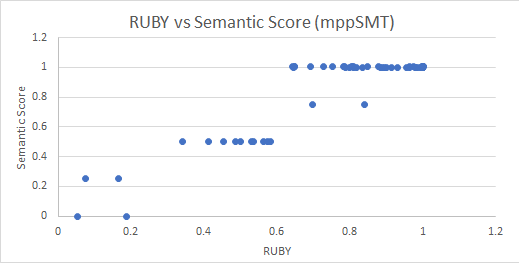
\includegraphics{img/rubyvssem_mppSMT.png}
\label{fig:RubySemMppSMT}
\end{figure}

As our experiment result, the correlation coefficients between {\model} and
semantic score are \textbf{0.764}, \textbf{0.815}, and \textbf{0.747} for the 3 models GNMT, mppSMT, and lpSMT  respectively. Comparing to the correlation of BLEU of 0.658, 0.523, and 0.570, {\model}'s results are much higher. 
In statistics, 
these values indicate a strong positive linear relationship between two 
quantitative metrics. That means one metric could be predicted by the other 
with high confidence. For example, an increase of 0.5, {\model} score can be 
interpreted as an increase of 0.4 in term of semantic score. Based on that 
information, developers can tune the SMT-based migration system in an incremental manner.

Figures~\ref{fig:RubySemlpSMT} and~\ref{fig:RubySemMppSMT} show the
scatter plots between {\model} and semantic scores on two models mppSMT
and lpSMT, respectively. For lpSMT (figure~\ref{fig:RubySemlpSMT}), 
there is a moderately strong, positive, linear association between the 
two variables with a few outliers. Beside, figure~\ref{fig:RubySemMppSMT} 
shows a strong, positive, linear association between {\model} and semantic 
score for the results translated by mppSMT. There are no outliers in the data. 
This indicates the result is consistent.

%In general, {\model} has high correlation with semantic scores. As our
%experiment result, the correlation coefficient between {\model} and
%semantic score for model mppSMT is \textbf{0.862} and for the model
%lpMSMP is \textbf{0.836}. In statistics, these values indicate a
%strong uphill linear relationship between two quantitative
%metrics. That means one metric could be predicted by the other with
%high confidence. For example, an increase of 0.5, {\model} score can
%be interpreted as an increase of 0.4 in term of Semantic score. Based
%on that information, developers can tune the system in an incremental
%manner.
%Specifically, a correlation of +0.8 implies that when 	

In general, the correlation coefficient between {\model} and semantic score cannot be 
stronger than GRS or even TRS. However, {\model} scores are available for any pair 
of the translated result and the reference code, while GRS and TRS are applicable for 
a subset of results. In our sample data, the sizes of these applicable set of methods
are quite small, for lpSMT they are \textbf{75/375} and \textbf{123/375}, and these figures
for mppSMT are \textbf{239} and \textbf{292} respectively. The summary results about correlation with semantic score is presented in \ref{fig:summary}

%While GRS is
%only computed with the migrated code with sufficient semantic
%information, {\model} does not depend on the code, even we can not parse
%PDGs and ASTs. This implies that there exist a {\model} score for any
%given code. On the other hand, in comparison with TRS, STS
%and BLEU, {\model} always outperforms the other three metrics.
\subsubsection{The use of {\model} in comparing models}
To evaluate {\model}'s abilities in comparing the translation quality
of models, we performed an evaluation of RUBY used in comparing
the two models mppSMT and p-mppSMT.
%examination to evaluate the effectiveness of {\model} in comparing
%mppSMT and p-mppSMT. 
%
Then, we also evaluated {\model} in comparing three real-world
SMT-based migration models lpSMT~\cite{fse13}, mppSMT~\cite{ase15},
and GNMT~\cite{gnmt}.  
%the effectiveness of {\model} is also evaluated in comparing several
%real-world translation models lpSMT, mppSMT and GNMT.
%
For any two models $M$ and $M'$, we proceeded as follows. First, we
performed $t$-test (at the confident level of 95\%) with the mean
values of the semantic scores on the two sets of results migrated by
the two models to compare them. We then processed $t$-test in the same
manner on the two sets of {\model}'s scores for the results migrated
by the two models to compare them. If the decision whether $M$ is
better than $M'$ by {\model} is consistent with that by the semantic
scores, we consider {\model} as effective in comparing the models.

%We use $t$-test and the mean values of semantic scores to conclude
%about the translation quality comparison between two models with a
%given confident level (95\% in our experiments).  The conclusion based
%on {\model} is also drawn in the same manner. The two conclusions will
%be checked whether consistent or not in order to confirm the
%effectiveness of {\model} in comparing these two models.


\textbf{Comparing mppSMT and p-mppSMT}. In this experiment, 
to compare the two models mppSMT and p-mppSMT, by using $t$-test, we
were able to reject the null hypothesis that \textit{the semantic
scores of two models are equal} with $p$-value of 2.81E-85 and the difference must be larger than 0.04 to be considered significant. Because the average semantic score of mppSMT
is greater than p-mppSMT by 0.268, we conclude that the translation
quality of mppSMT is better than p-mppSMT based on the semantic
scores.
%
To compare mppSMT and p-mppSMT using {\model}, we performed an
$t$-test with the null hypothesis that \textit{the {\model} scores of
two models are equal}. We were able to reject it with $p$-value of
7.78E-65 ant t-critical value of 1.97 at 95\% confident interval. For mppSMT, the mean value of {\model} scores is higher than
that of p-mppSMT (0.258). Hence, the conclusion that mppSMT is better
than p-mppSMT is consistently stated by {\model} and by the semantic
scores.
%based on {\model} and semantic score are consistent. 
Thus, we conclude that the effectiveness of {\model} in comparing
mppSMT and p-mppSMT is confirmed.
%{\model} is able to identify their difference 
%in translation quality estimated by semantic similarity. Specifically, the model mppSMT's 
%average {\model} score is higher than p-mppSMT by \textbf{0.258} which nearly equals 
%to the difference in term of semantic score (0.268). We also perform t-test on the data 
%set to see if there is a significant difference in 
%{\model} scores. With confident level of 0.95, we get the p-value of 7.78E-65. 
%That means, we reject the null hypothesis and conclude that mppSMT's {\model} 
%score is higher than p-mppSMT's ones.

\textbf{Comparing real-world models}. We also perform experiments to compare the three models 
lpSMT, mppSMT and GNMT in pairwise. The $p$-values with the null hypothesis \textit{the semantic 
scores of two models are equal} and the mean values for the translated results of three models 
are shown in table \ref{table:tTestResult}  and table \ref{table:avgRubySem}  For all pairs of models, {\model} shows consistent results with semantic scores. An improvement in {\model} scores when comparing between models always equivalents to an improvement in translation quality represented by semantic scores.  
%For each pair of models, we perform t-test on their 
%semantic scores to test whether there is a significant difference between them. 
%If yes, then the average semantic scores are used to determine if a model has higher 
%semantic score than another. The same process is applied to {\model} score. The 
%\ref{table:rubyCross} demonstrates our result. In all the pairs, {\model} can measure 
%the difference of semantic scores between models. 
%Comparing models GNMT and mppSMT, we found out that in \textbf{97.7\%} of the cases, the change in {\model} score indicates the change in the same direction for Semantic score. It means an improvement in {\model} score equivalents an improvement in Semantic scores and vice versa. More interestingly, 83 of 88 cases (\textbf{94.3\%}) if a pair of translated results have the same Semantic score, they also have identical {\model} score. 
%As the results showing, {\model} is a reliable metric to use in comparing different SMT-based migration models. 
\begin{table}
\centering
\caption{P-value Results}
\begin{tabular}{|c|c|c|c|}
\hline
 & GNMT \& mppSMT & lpSMT \& mppSMT & lpSMT \& GNMT \\
\hline
Semantic  & 1.70E-35 & 3.32E-4 & 3.22E-26  \\
\hline
RUBY  & 2.27E-25 & 1.10E-3 & 9.72E-26  \\

\hline
\end{tabular}
\label{table:tTestResult}
\end{table}

\begin{table}
\centering
\caption{Average semantic and RUBY scores}
\begin{tabular}{|c|c|c|c|}
\hline
 & GNMT & lpSMT & mppSMT \\
\hline
Semantic average & 0.714 & 0.879 & 0.914  \\
\hline
{\model} average & 0.743 & 0.886 & 0.905  \\
\hline
\end{tabular}
\label{table:avgRubySem}
\end{table}


	    
\begin{figure}
\centering
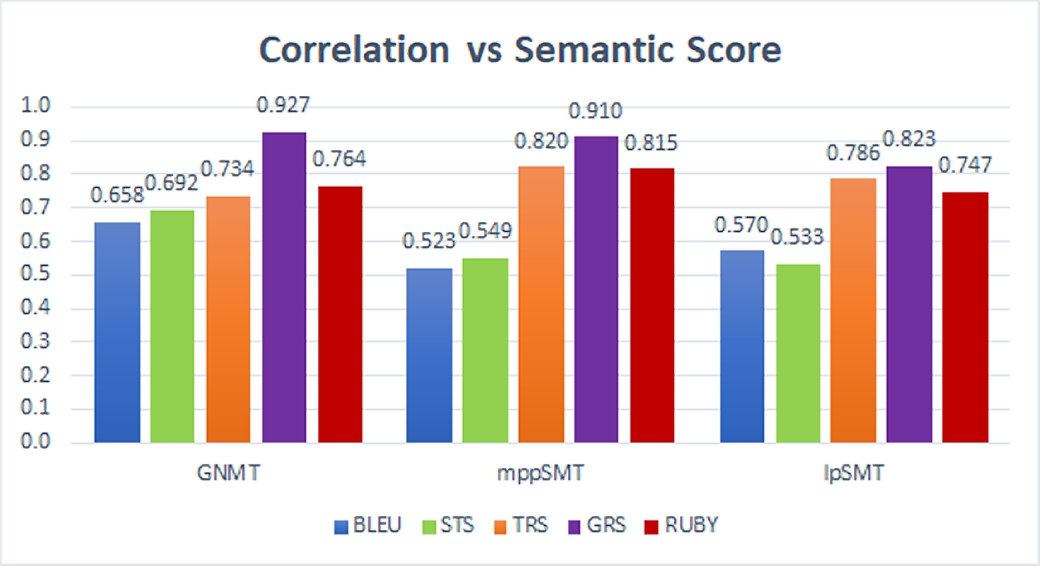
\includegraphics[scale=0.85]{img/summary.jpg}
\label{fig:summary}
\end{figure}